\documentclass[11pt]{article}

\usepackage[margin=1in]{geometry}
\usepackage{amsmath,amssymb,amsthm}
\usepackage{mathtools}
\usepackage{enumitem}
\usepackage{xcolor}
\usepackage{graphicx}
\graphicspath{{Vlasov/formalize/retrospective/}}
\usepackage{hyperref}
\hypersetup{colorlinks=true,linkcolor=blue!50!black,citecolor=blue!50!black,urlcolor=blue!50!black}

% --- environments -----------------------------------------------------------
\theoremstyle{plain}
\newtheorem{theorem}{Theorem}[section]
\newtheorem{lemma}[theorem]{Lemma}
\newtheorem{proposition}[theorem]{Proposition}
\theoremstyle{definition}
\newtheorem{definition}[theorem]{Definition}
\newtheorem{strategy}{Strategy}[section]
\theoremstyle{remark}
\newtheorem{remark}[theorem]{Remark}

% --- notation ---------------------------------------------------------------
\newcommand{\R}{\mathbb{R}}
\newcommand{\N}{\mathbb{N}}
\newcommand{\Wone}{W_1}
\newcommand{\Wbar}{\overline{W}}
\newcommand{\lean}[1]{\texttt{#1}}
\newcommand{\printaxioms}{\lean{\#print axioms}}
\newcommand{\cleanfootprint}{\lean{[propext,\,Classical.choice,\,Quot.sound]}}

\title{\textbf{Mathematician in the Loop}\\[2pt]
\large AI-assisted Lean formalization as a strategy game,\\
with a worked end-to-end case study in kinetic theory}

\author{Joseph K. Miller
}
\date{\today}

\begin{document}
\maketitle

\begin{abstract}
We describe a methodology for formalizing research mathematics in the Lean~4
proof assistant, in which a human mathematician guides an AI agent system
through an extended interactive session. We frame the activity as a
\emph{game}: the objective is to turn a \LaTeX{} mathematics document into a
Lean development; the game is \emph{won} when the development compiles with no
\lean{sorry} and \printaxioms{} on the target theorems returns only Lean's
foundational axioms; and each won game carries a \emph{score} measuring how much
of the resulting code is reusable --- operationally, how much of the
development can be extracted as a clean, dependency-isolated, upstreamable
library layer. We argue the game has three phases with genuinely distinct
optimal strategies --- an \emph{early game} dominated by definitional scoping, a
\emph{mid game} dominated by human-judgment proof decomposition, and an
\emph{end game} dominated by the triage of gaps against the ambient library's
coverage --- and we present a taxonomy of reusable guidance strategies (the
$\mathrm{P}/\mathrm{L}/\mathrm{M}/\mathrm{B}$ series) that the human encodes into
the agent's standing instructions as the game proceeds.

We demonstrate the method on a substantial case study: a complete, axiom-clean
formalization of well-posedness for the Vlasov equation via Dobrushin's
mean-field route --- existence, uniqueness, the mean-field stability estimate,
and the mean-field limit --- at \emph{arbitrary} interaction-Lipschitz constant.
The target theorems depend only on Lean's three foundational axioms; the
optimal-transport machinery built along the way (a finite Kantorovich duality, a
transport-polytope compactness theory, a coupling-gluing construction) is
separated into a self-contained layer with a four-name interface to the
kinetic-theory content. We report the methodology candidly, including the
mode in which ``about a week'' is the honest figure: a human mathematician
acting as strategic director over an AI execution engine, with a verification
discipline that keeps the development sound at speed.
\end{abstract}

\tableofcontents

% ============================================================================
\section{Introduction}
% ============================================================================

\paragraph{The problem.}
Formalizing frontier mathematics in a proof assistant is slow, and the
bottleneck is rarely the proof assistant's logic. It is the sheer volume of
intermediate lemmas, the friction of matching an informal argument to the
ambient library's idioms, and --- for analysis in particular --- the gaps in
that library's coverage of functional-analytic infrastructure. A research
paper that a human reads in an afternoon can take a skilled formalizer weeks to
mechanize. Modern AI agents can write Lean proofs, but left to themselves they
do not know \emph{which} lemma to prove next, \emph{how} to cut a hard theorem
into tractable pieces, or \emph{when} a missing fact is a genuine library gap
versus an artifact of the wrong proof strategy. Those are mathematical
judgments.

\paragraph{The proposal.}
We put the mathematician back in the loop. The human does not write the Lean;
the human \emph{directs} an AI agent system --- here, an agentic coding
environment with access to the source \LaTeX{} document, the Lean files being
written, and a standing instruction file (\lean{CLAUDE.md}) that governs the
agent's behavior. The human's contribution is strategic: scope the definitions,
choose the decompositions, triage the gaps, and --- crucially --- distill
recurring strategic insights into reusable guidance that the agent internalizes
through its standing instructions. We found this division of labor productive
enough to formalize a genuine research result end to end in roughly a week of
calendar time, and we believe the \emph{structure} of how that worked is worth
reporting independently of the result.

\paragraph{The framing.}
We describe the activity as a game because the framing is unusually faithful.
There is a precise objective (turn the \LaTeX{} into Lean), a precise and
machine-checkable win condition (zero \lean{sorry}, clean axiom footprint), and
a meaningful score (reusability of the won code). And there are three phases,
each with a different dominant strategy --- the same player who excels at the
opening can lose the endgame by playing it with opening heuristics. Making the
phases explicit, and naming the strategies that win each one, is the
contribution of this paper.

\paragraph{Outline.}
Section~\ref{sec:game} formalizes the game, its win condition, and its score.
Section~\ref{sec:phases} describes the three phases and their dominant
strategies. Section~\ref{sec:strategies} presents the
$\mathrm{P}/\mathrm{L}/\mathrm{M}/\mathrm{B}$ strategy taxonomy --- the standing
guidance the human accumulates and the agent internalizes.
Section~\ref{sec:casestudy} is the worked Vlasov case study, with the key
definitions, theorems, and the genuinely hard lemmas presented as instances of
the three phases. Section~\ref{sec:discipline} describes the verification
discipline that keeps the method sound. Section~\ref{sec:assessment} assesses
the methodology, including an honest account of the ``about a week'' figure and
the reusability score actually achieved.

% ============================================================================
\section{The game}\label{sec:game}
% ============================================================================

\subsection{Objective, win condition, score}

\begin{definition}[The formalization game]\label{def:game}
The game is played on a triple $(\mathcal{T}, \mathcal{L}, \mathcal{G})$ where
$\mathcal{T}$ is a source mathematics document (a \LaTeX{} paper),
$\mathcal{L}$ is a Lean~4 development under construction, and $\mathcal{G}$ is a
standing instruction file governing the agent's behavior. A distinguished set
of \emph{target theorems} $\Theta \subseteq \mathcal{L}$ encodes the main
results of $\mathcal{T}$. The human and the agent system alternate moves that
edit $\mathcal{L}$ and $\mathcal{G}$.
\end{definition}

\begin{definition}[Win condition]\label{def:win}
The game is \emph{won} when:
\begin{enumerate}[label=(W\arabic*),leftmargin=3em]
\item $\mathcal{L}$ compiles, with no occurrence of \lean{sorry} in any
declaration reachable from $\Theta$; and
\item for every $\theta \in \Theta$, the command \printaxioms{}~$\theta$
returns exactly \cleanfootprint.
\end{enumerate}
\end{definition}

The second clause is the substantive one, and it is the reason we frame the win
condition in terms of the \emph{axiom footprint} rather than the more obvious
``no \lean{sorry}.'' A development can be free of \lean{sorry} and still depend
on a bespoke \lean{axiom} declaration --- a \lean{sorry} renamed to look
principled. Lean's \printaxioms{} traces the \emph{complete} set of axioms a
theorem transitively depends on; the three names \lean{propext},
\lean{Classical.choice}, and \lean{Quot.sound} are Lean's own foundations, and
nothing else. A theorem whose footprint is exactly these three is proved
``modulo Lean's foundations alone.'' Any fourth name --- a \lean{sorryAx} from a
hidden \lean{sorry}, a custom axiom, a deferred placeholder --- is a loss, and
the footprint check catches it where a build-success check would not. The win
condition is therefore not ``the code compiles'' but ``the code compiles
\emph{and} the foundations are clean,'' and these are different claims
(see Strategy~\ref{strat:P10}).

\begin{definition}[Reusability score]\label{def:score}
A won game is scored by the \emph{extractability of its general layer}: the
fraction of $\mathcal{L}$ that can be carved into a self-contained sub-library
$\mathcal{L}_{\mathrm{gen}}$ such that
\begin{enumerate}[label=(S\arabic*),leftmargin=3em]
\item $\mathcal{L}_{\mathrm{gen}}$ contains no problem-specific declarations
(it is general mathematics, not about $\mathcal{T}$'s specific objects);
\item the dependency graph admits a one-directional cut: every edge between
$\mathcal{L}_{\mathrm{gen}}$ and the rest crosses a small, explicit interface,
and no declaration in $\mathcal{L}_{\mathrm{gen}}$ depends on a
problem-specific one; and
\item the declarations in $\mathcal{L}_{\mathrm{gen}}$ are named and structured
to the ambient library's conventions --- they could be submitted upstream with
cosmetic edits only.
\end{enumerate}
\end{definition}

This score is concrete and measurable rather than aesthetic. Clauses (S1) and
(S2) are decided by the development's declaration-level dependency graph, which
can be extracted from the proof assistant's own elaboration environment.
Clause (S3) is decided by a naming-and-structure audit. In the case study
(Section~\ref{sec:casestudy}) the general layer is the optimal-transport
machinery, the interface to the problem-specific (kinetic-theory) content is
exactly four names, and the audit passed on all $56$ declarations of the
extracted layer.

\subsection{Why ``game'' is the right metaphor}

Three features make the metaphor load-bearing rather than ornamental. First,
the win condition is \emph{adversarial in a specific sense}: the proof assistant
will not be fooled. Unlike informal mathematics, where a gap can hide in a
``clearly,'' a Lean development that wins Definition~\ref{def:win} is checkable
by a referee in seconds (run the build; run \printaxioms{}). The opponent is
the type-checker, and it does not accept hand-waving.

Second, the score creates a genuine trade-off. The fastest path to (W1)--(W2)
is often to prove everything in the most problem-specific form available;
the highest-scoring path requires building general infrastructure and keeping it
dependency-clean. A player optimizing only for the win will under-invest in
reusability; a player optimizing only for the score may never finish. Good play
balances them, and the balance shifts by phase.

Third --- and this is the part that motivates the rest of the paper --- the
phases reward \emph{different} strategies, and carrying an early-game strategy
into the endgame is a characteristic way to lose.

% ============================================================================
\section{The three phases}\label{sec:phases}
% ============================================================================

\subsection{Early game: definitional scoping}

In the early game the player translates the main theorems of $\mathcal{T}$ into
Lean theorem \emph{statements}, with proofs left as \lean{sorry}. This sounds
mechanical and is not. The difficulty is not the theorem statements; it is the
\emph{definitions of the objects} those statements quantify over. Every later
move builds on these definitions, so a definition that is subtly wrong --- one
that bakes in the wrong hypothesis, the wrong metric, or the wrong regularity
class --- propagates its error through the entire development and is most
expensive to discover late.

\begin{quote}\itshape
The early-game risk is definitional. The dominant strategy is to lock the
object scaffolding --- the definitions and the target signatures --- before
proving anything, and to read the source document at the level of atoms (which
exact hypothesis, which exact moment, which exact norm) rather than at the level
of prose.
\end{quote}

Concretely, the player commits the \emph{statements} of the target theorems and
the definitions they reference, gets the file to compile with every proof a
\lean{sorry}, and only then begins to prove. This ``API-lock'' (Strategy
\ref{strat:P4}) separates the act of committing to an interface from the act of
discharging it, which matters because the interface is what every subsequent
phase is written against. Errors caught here are cheap; the same errors caught
in the endgame require unwinding everything built on top.

\subsection{Mid game: human-judgment decomposition}

In the mid game the player repeatedly takes a sorried statement and
\emph{decomposes} it into smaller sorried sub-statements, each heuristically
easier, until the leaves are within reach of the agent's proving ability. This
is where, in the language of the project, ``the mathematician's hat goes on.''

The central empirical claim of this paper is that \textbf{decomposition is the
irreducibly human-judgment part of the loop.} An AI agent can prove a
well-specified sub-lemma; what it does poorly is \emph{choose} the decomposition
that makes the original problem tractable --- which sub-problems are
heuristically easier, where to cut, which of several equivalent routes leads to
a proof the library can actually support. Those are acts of mathematical taste.
In the case study, the decisive mid-game choices were exactly of this kind:
routing the mean-field stability estimate through an infimum-over-couplings
inequality (which needs no attainment theorem) rather than through optimal-coupling
attainment; choosing a discrete-approximation route to Kantorovich duality over
a Hahn--Banach route; cutting the coupling triangle inequality through a
disintegration-and-gluing construction. Each was a human decision; each was then
executed by the agent.

The mid game also has a \emph{learning} component, and it is the reason the
standing instruction file $\mathcal{G}$ is a live part of the game rather than a
fixed prompt. When the human recognizes a recurring decomposition pattern --- or,
more often, a recurring \emph{failure} pattern --- they distill it into a
strategy and write it into $\mathcal{G}$, where the agent internalizes it for
all subsequent moves. The loop thus accumulates the human's strategic insight
as standing guidance. Section~\ref{sec:strategies} is the taxonomy of strategies
that accumulated this way.

\begin{quote}\itshape
The mid-game risk is choosing a decomposition the library cannot support, or one
that multiplies rather than reduces difficulty. The dominant strategy is
human-selected decomposition --- cut where the mathematician sees tractability ---
combined with encoding each hard-won decomposition heuristic into $\mathcal{G}$
so it is reused, not re-derived.
\end{quote}

\subsection{End game: triaging the library gaps}

Eventually the development reaches sorried statements that are not further
decomposable into project-specific pieces --- they are requests for
\emph{general} mathematics that the ambient library may or may not contain. For
the formalization of partial differential equations, this phase has a specific
character: it becomes the work of \textbf{understanding what functional-analytic
gaps are present in the library}, and deciding what to do about each.

The surviving sorries partition into three kinds, and the endgame is the triage:
\begin{enumerate}[label=(\alph*),leftmargin=2.5em]
\item \emph{Phantoms}: statements that look like genuine gaps but dissolve under
a sharper reading of what the consumer actually needs. In the case study, an
entire conjectured ``foundation'' (a metrization theorem relating narrow and
$\Wone$ convergence) turned out to be a phantom: the one consumer needed only
the easy lower-semicontinuity half of it, which is a short, library-supported
lemma. The work here is recognizing that the gap is not real before building
to fill it.
\item \emph{Genuine gaps you build}: standard mathematics the library lacks,
which the player decides to formalize from the primitives that \emph{are}
present. In the case study this was finite Kantorovich duality, built from the
library's Farkas lemma.
\item \emph{Genuine gaps you honestly defer}: standard mathematics the library
lacks, which the player marks with an explicit, cited placeholder rather than
building --- when the cost of building outweighs the value, and the dependency
is on a recognized, true theorem.
\end{enumerate}

\begin{quote}\itshape
The end-game risk is misclassifying: building infrastructure for a phantom, or
silently assuming a gap that should be marked. The dominant strategy is triage
against the library's actual coverage --- which requires knowing the library at
the functional-analysis level --- and verifying each candidate gap at the level
of what the consumer truly needs before committing to build it.
\end{quote}

This phase is, we think, an under-appreciated structural fact about formalizing
research analysis: progress is rate-limited by the ambient library's
infrastructure, and the endgame is precisely the work of locating, and either
filling or honestly marking, the places where that infrastructure runs out.

% ============================================================================
\section{The strategy taxonomy}\label{sec:strategies}
% ============================================================================

The standing instruction file accumulated, over the course of the game, a set of
lessons organized into four series. The series are not arbitrary: they operate
at genuinely different levels, with different triggers for ``this rule applies''
and different audiences in the agent's reasoning when it consults them.

\begin{description}[leftmargin=2em,style=nextline]
\item[L-series --- Lean / agent-tool lessons.] Idioms, elaborator quirks,
parser quirks, and the engineering of agent sub-task specifications. Consulted
at the level of writing or debugging an individual Lean proof.
\item[P-series --- Process discipline.] When to ask, when to commit, when to
delegate, when to pivot, how to verify. Consulted at the per-move discipline
level, and whenever a tactical plan starts surfacing repeated friction.
\item[M-series --- Mathematical structure.] Principles about which mathematical
structures to work in and what shape a proof should take. Consulted when
designing a proof before writing it.
\item[B-series --- Bridging architecture.] When to introduce new infrastructure
versus patch an existing seam. Consulted when frictions accumulate across
several attempted bridges.
\end{description}

We state a representative strategy from each series; these are the ones that
recurred most and did the most work in the case study.

\begin{strategy}[P4: API-lock vs.\ substantive proof]\label{strat:P4}
When a theorem's body requires a multi-step composition that exceeds a single
working session, do not inline the full composition. Instead, commit the
\emph{signature} of the theorem and of its named sub-lemmas first --- with
sorried bodies --- and verify that the composition typechecks against the locked
interfaces before discharging any body. This separates interface commitment from
proof discharge, prevents a proliferation of sub-sorries inside an un-checkpointable
inline block, and lets each leaf be proved and committed independently.
\end{strategy}

\begin{strategy}[P5: the framework's own extrapolations need atom-level
verification]\label{strat:P5}
The strategy framework itself recognizes patterns and produces recommendations
(``this looks like the situation where X''). Such a recommendation is a
\emph{hypothesis to verify}, not a conclusion to act on. Before executing a
pattern-extrapolated plan, read the actual artifacts at the atom level
(the exact construction, the exact dependency, the exact hypothesis) and confirm
the pattern truly applies. The case study repeatedly found that the
``obvious'' reading was wrong in a way only an atom-level read exposed --- the
phantom foundation, a stale planning note that confidently asserted a dead-end
route, a hidden reach-slack in a tiling argument.
\end{strategy}

\begin{strategy}[P10: a green build permits multiple stories; only an audit
certifies]\label{strat:P10}
After a non-trivial refactor, a clean build is necessary but not sufficient for
``the refactor preserved meaning.'' The build certifies typechecking against the
new types; it does not certify that consumers use the new types for the same
mathematical purpose. The certifying instrument is \printaxioms{}: it traces the
complete axiom dependency and exposes any hidden \lean{sorry} or custom axiom.
Trust the footprint, not the green build --- and never trust an automated agent's
report of success without re-running the footprint check by hand.
\end{strategy}

\begin{strategy}[P11: a check that ran against a failed build is stale]\label{strat:P11}
A move followed by ``build, then footprint-check'' can mislead: if the build
\emph{fails}, the footprint check may still print a passing result, because it
ran against the previous build's cached artifacts. Reading that pass as success
is a false certification --- it certifies the \emph{old} state, not the current
edit. Always confirm the build succeeded \emph{before} trusting any secondary
check.
\end{strategy}

\begin{strategy}[M3/M4: distinguishing artifact constraints from genuine
ones]\label{strat:M}
A smallness constraint imposed by a \emph{static} construction forcing a
parameter to bound its own growth is an \emph{artifact} that dissolves when the
construction is rebuilt on the sharp time-local bound; a constraint from a
genuine analytic mechanism (a contraction ratio below one) does not. When
removing a constraint imposed by chaining or tiling short pieces, use
\emph{exact} tiling rather than naively dropping the offset in the bound ---
because the chain may overshoot the target by a reach-slack the interface does
not expose, producing a threshold that looks general but is secretly
data-dependent --- and certify the removal by instantiating the formerly
forbidden parameter value and confirming it typechecks.
\end{strategy}

\begin{strategy}[B3: conjunct shape is bounded below by the consumer, above by
the producers]\label{strat:B3}
When strengthening a predicate with a new conjunct, the conjunct's strength is
bounded below by what the consumer needs and above by what \emph{every} producer
can supply. Read both the consumer and all producers before fixing the
conjunct's shape: reading only the consumer can leave it over-strong for some
producer to satisfy; reading only the producers can leave it under-strength.
\end{strategy}

A point worth emphasizing about the taxonomy: these strategies were not designed
in advance. They were \emph{earned}, each one keyed to a specific failure that
occurred during the game and was then encoded into $\mathcal{G}$ to prevent its
recurrence. The standing instruction file is, in effect, a record of the
mathematician's accumulated strategic experience, written in a form the agent
can consult. This is the mechanism by which the human's judgment is amortized
across the thousands of individual moves the agent makes.

% ============================================================================
\section{Case study: well-posedness for the Vlasov equation}\label{sec:casestudy}
% ============================================================================

We played the game on Dobrushin's derivation of the Vlasov equation from
$N$-particle Hamiltonian dynamics. This section presents the key definitions and
target theorems, then the genuinely hard lemmas, organized by the phase in which
each arose.

\subsection{Setting and key definitions}

Phase space for a single particle in spatial dimension $d$ is
$\mathbb{X} := \R^d \times \R^d$ (position and velocity). The pair potential
$W : \R^d \to \R$ satisfies a standing assumption (in the development, the type
class \lean{AssW}): $W$ is continuously differentiable, even, and has a globally
Lipschitz gradient with constant $L := \mathrm{Lip}(\nabla W)$.

\begin{definition}[Wasserstein-1 distance]
For probability measures $\mu,\nu$ with finite first moment on a metric space,
$\Wone(\mu,\nu)$ is the optimal-transport cost for the ground cost
$c = \mathrm{dist}$. The development carries two faces of this object: the
\emph{dual} form (a supremum over $1$-Lipschitz test functions) and the
\emph{primal} form (an infimum over couplings). It also carries the truncated
variant $\Wbar$ with ground cost $\min(\mathrm{dist},1)$, used in the analysis of
the global-in-time argument.
\end{definition}

\begin{definition}[Newton and Vlasov dynamics]
The $N$-particle mean-field Newton system is
\[
\dot{x}_i = v_i, \qquad
\dot{v}_i = -\tfrac{1}{N}\sum_{j\neq i} \nabla W(x_i - x_j),
\qquad i = 1,\dots,N,
\]
and the Vlasov equation is the kinetic mean-field limit, whose characteristic
flow transports a measure $\rho_t$ along the self-consistent force field
$-(\nabla W * \rho_t)$.
\end{definition}

\subsection{The target theorems}

\begin{theorem}[Well-posedness, \lean{vlasovWellPosedness}]\label{thm:wp}
Under the standing assumption on $W$ \emph{(at arbitrary Lipschitz constant
$L$)}, the Vlasov characteristic flow exists and is unique, globally in time.
\end{theorem}

\begin{theorem}[Mean-field stability and limit, \lean{dobrushin}]\label{thm:dob}
Two Vlasov solutions are stable in $\Wone$ with an explicit (Gronwall) rate, and
the empirical measures of the $N$-particle Newton dynamics converge to the
Vlasov solution in the mean-field limit.
\end{theorem}

Both theorems are \emph{won} in the sense of Definition~\ref{def:win}:
\printaxioms{} on each returns exactly \cleanfootprint. We highlight that
Theorem~\ref{thm:wp} holds at arbitrary $L$ --- the small-$L$ restriction present
in a naive formalization of Dobrushin's argument is removed
(Section~\ref{ssec:endgame-lemmas}).

\subsection{Early-game lemmas: getting the definitions right}

The early game's substance was definitional, and one example shows why it
matters. The Wasserstein cost is defined generically over the ground cost $c$;
the development carries cost-generic property lemmas (symmetry, triangle
inequality) and then instantiates them at $c = \mathrm{dist}$ (for $\Wone$) and
$c = \min(\mathrm{dist},1)$ (for $\Wbar$). Locking this cost-generic interface
\emph{first} --- before proving any analytic content --- meant that the later
introduction of $\Wbar$ for the global-in-time argument was an instantiation,
not a re-derivation. A development that hard-coded $\mathrm{dist}$ into the
Wasserstein definitions would have paid for it in the endgame.

A subtler early-game point (an instance of Strategy~\ref{strat:B3}): a coupling
cost bound needs a moment hypothesis stated against the \emph{ground cost} $c$,
not against $\mathrm{dist}$; at the instantiation $c=\mathrm{dist}$ the two
coincide definitionally, but stating the lemma against the wrong one makes its
proof impossible while leaving the marquee instantiation looking fine. Reading
both the consumer's need and every producer's capacity --- before freezing the
hypothesis --- is what caught this.

\subsection{Mid-game lemmas: decomposition choices}

\paragraph{The dual/primal split (the decisive decomposition).}
The mean-field stability estimate (Theorem~\ref{thm:dob}) is naturally stated in
the dual $\Wone$. Proved directly, it appears to require an \emph{optimal
coupling} --- an attainment theorem the library does not have. The decomposition
that unlocked the proof was to state the stability core in the \emph{primal}
coupling cost and discharge it by an infimum-over-couplings inequality (``the
infimum is below \emph{any} particular coupling's cost''), which needs no
attainment. The dual-form headline is then recovered as a one-line corollary
through a single bridge lemma identifying the two faces of $\Wone$. This
relocated the only genuine optimal-transport dependency to one labeled line, and
left the entire dynamical content --- existence, uniqueness, the stability core,
the mean-field limit --- provably independent of it.

\paragraph{The coupling triangle inequality (a disintegration gluing).}
The primal coupling cost satisfies a triangle inequality, and its proof is a
genuinely delicate measure-theoretic construction: given a coupling of
$(\mu,\rho)$ and a coupling of $(\rho,\nu)$, one disintegrates the second over
$\rho$ and glues, producing a coupling of $(\mu,\nu)$. The load-bearing and
error-prone part is not the cost bound --- it is proving the glued measure has
the \emph{correct marginals}, i.e.\ that it is genuinely a coupling of
$(\mu,\nu)$. Marginal-preservation through the disintegration-and-recombination
is exactly where a ``near-citation'' from the library hides a gap; the cost
bound is the easy half. (This is why the coupling triangle inequality requires a
ground-cost triangle hypothesis that the dual-side triangle inequality does
not.)

\subsection{End-game lemmas: the library gaps}\label{ssec:endgame-lemmas}

\paragraph{The phantom foundation.}
The development initially carried two conjectured ``foundations'' as external
gaps. One --- a metrization theorem relating narrow convergence and $\Wone$ ---
turned out to be a phantom. The single consumer needed only the easy
lower-semicontinuity direction (Villani's lower-semicontinuity of $\Wone$ under
narrow convergence with moment control), which is a short lemma provable from the
dual representation. The full metrization was never load-bearing; recognizing
this --- before building it --- is the endgame's triage in action. The
certification confirmed it: with the metrization never invoked, the target
theorems' axiom footprint was already clean of it.

\paragraph{Finite Kantorovich duality from Farkas (the genuine gap, built).}
The one genuine optimal-transport external --- the hard direction of the
Kantorovich--Rubinstein duality, on finitely-supported measures --- has no
packaged form in the library. We built it. The route had a fork the library
forced: the natural map-form of the duality lives on a Hilbert space and ran into
systemic friction between the proof assistant's inner-product instances on its
Euclidean space type; pivoting to the geometric separation on the plain product
$\iota \to \R$ (continuous linear functionals, no inner products) removed the
friction. We also confirmed the appealing Birkhoff-vertex shortcut was blocked:
the library has the doubly-stochastic (uniform-marginal) Birkhoff theorem, but
the transportation polytope here has general marginals and no library theory.
The surviving route assembled the library's Farkas lemma (conic separation) with
two compactness facts we proved by hand (primal attainment on the transport
polytope; closedness of the image cone) and a $c$-transform converting the dual
pair into a single admissible potential. The metric structure (triangle,
symmetry) enters \emph{only} in the $c$-transform; the linear-programming duality
itself is metric-free. The whole construction yields the duality \emph{inequality}
the consumer needs --- not an attained optimum --- consistent with the dynamical
content never requiring attainment.

\paragraph{Removing the small-$L$ restriction (exact tiling).}
A naive formalization of Dobrushin's global-in-time argument requires the
interaction Lipschitz constant to be small ($L<1$), inherited from a per-window
construction with a fixed unit force-window. Tracing the dependency to its single
structural origin showed that the offending small-$L$ threshold arose from the
window construction's unit width, not from any genuine analytic mechanism (an
instance of Strategy~\ref{strat:M}). The fix was \emph{exact} tiling: cover the
target interval with $N$ windows of width exactly $T/N$, so the chain lands
exactly on the target. Crucially, the naive alternative --- ``drop the $+1$
offset, replace $(T+1)^2$ by $T^2$'' --- would have left a hidden reach-slack
$(T+\delta)$ from the last window's overshoot, producing a threshold that
\emph{looks} general but fails for large $L$. The construction was rebuilt with
exact tiling, and the removal was certified the right way: by instantiating the
theorem at $L=2$ (a formerly forbidden value) and confirming it typechecks with
no smallness hypothesis.

\subsection{The reusability outcome}

After the game was won, we extracted the optimal-transport machinery into a
self-contained layer (Definition~\ref{def:score}). The declaration-level
dependency graph confirmed the separation: the kinetic-theory content reaches
the optimal-transport layer through exactly four names, and no
optimal-transport declaration depends on any kinetic-theory declaration. A
naming audit of all $56$ declarations in the extracted layer found them free of
project-specific jargon and in the ambient library's conventional shape. The
extraction was performed move by move, with the axiom footprint re-verified after
each move to confirm the reorganization changed only \emph{where} declarations
live, never \emph{what} the target theorems depend on. The layer --- a finite
Kantorovich duality, a transport-polytope compactness theory, a coupling-gluing
construction, and the $\Wone/\Wbar$ and coupling API --- is a candidate upstream
contribution in its own right, independent of the kinetic-theory application that
motivated it.

\paragraph{A human-auditable cross-check.}
Independently of the declaration-level graph used to compute the score, the
development carries a \emph{blueprint}: each marquee and infrastructure result is
tagged in the Lean source, and a build step extracts a dependency graph whose edges
are read directly from the elaborated proof terms (not hand-drawn), attaches to each
node its statement and an informal proof sketch, and links it to the formal
declaration and its \lean{leanok} (``formalized'') marker.
Figure~\ref{fig:depgraph} reproduces that graph. It is a coarser, theorem-level view
than the declaration-level graph, but it independently exhibits the same
architecture: the optimal-transport machinery (left) feeds the marquee
\lean{dobrushin} with no edge in the reverse direction --- the one-directional cut
the score formalizes --- while the kinetic-theory and superposition-bridge content
(right) feeds \lean{vlasov-wp} and the superposition principle. Every node is green:
the entire graph is formalized, with no informal placeholder on any path to a target.

\begin{figure}[t]
\centering
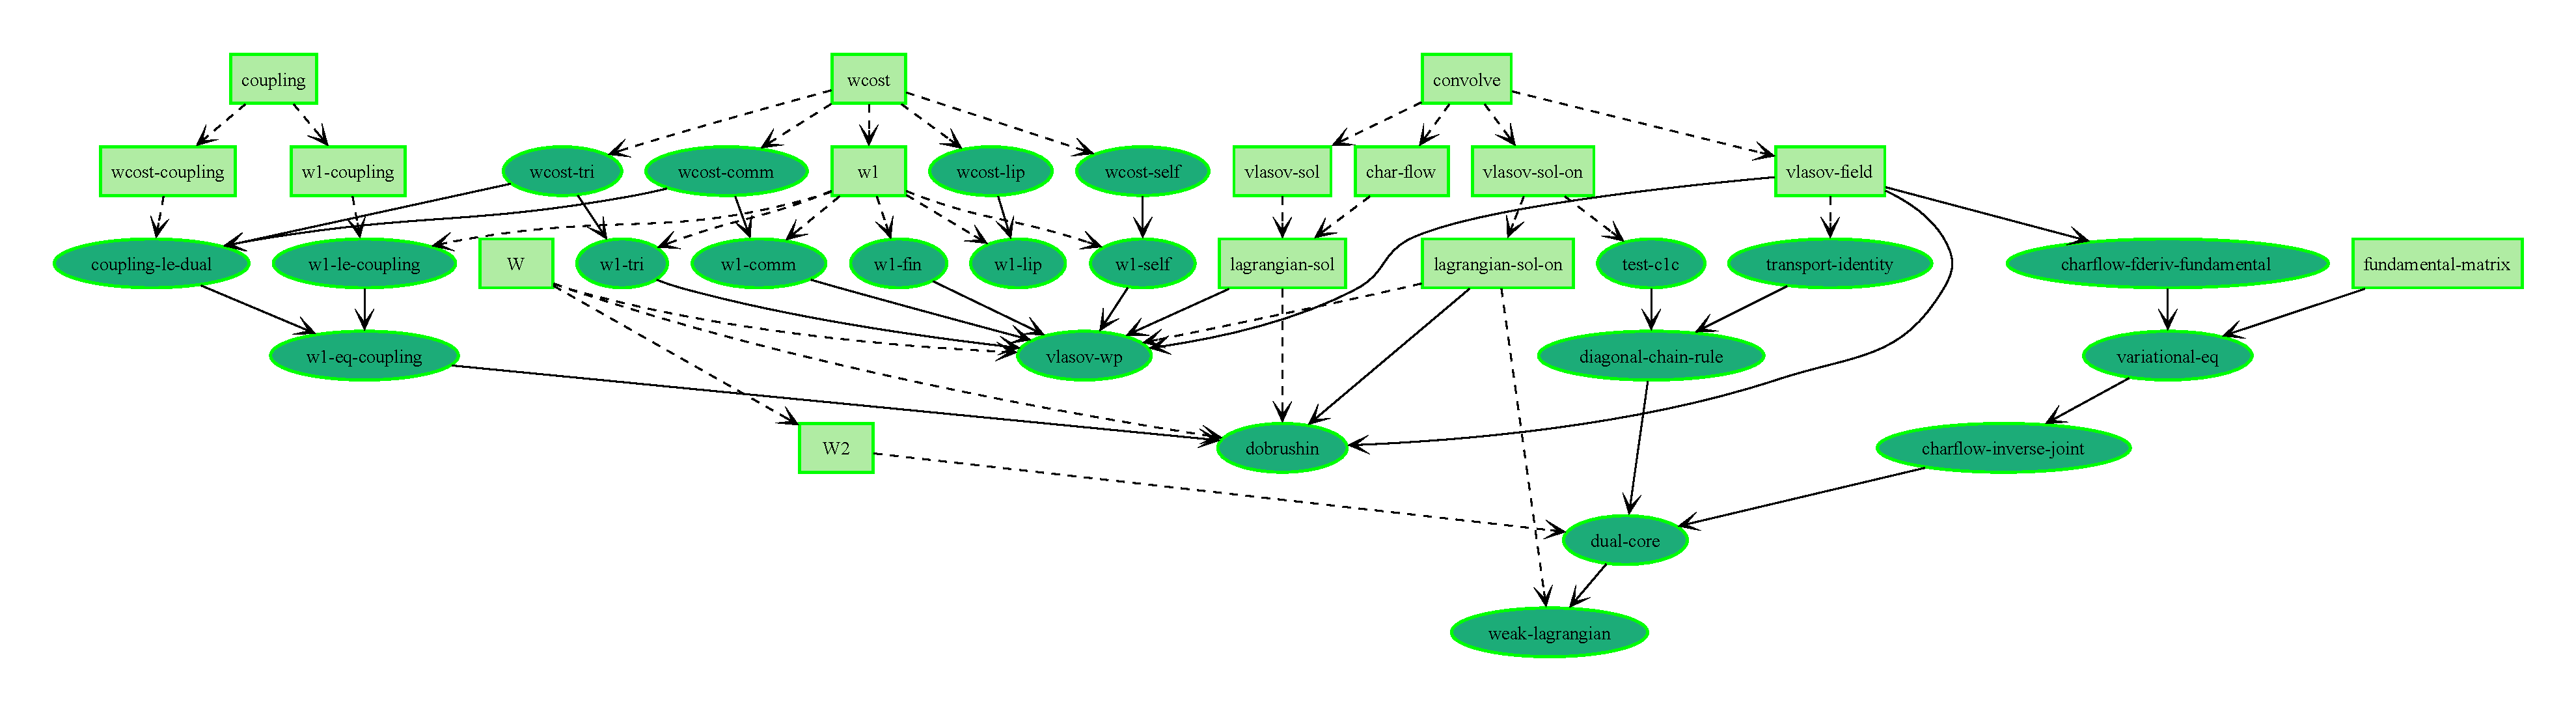
\includegraphics[width=\textwidth]{blueprint_depgraph.pdf}
\caption{The project blueprint's dependency graph, auto-extracted from the
elaborated Lean proof terms. Box nodes are definitions and assumptions, ellipse
nodes are theorems; dashed edges are statement-level dependencies and solid edges
proof-level dependencies; green marks a fully formalized (\lean{leanok}) node. The
optimal-transport layer (left, the \lean{wcost}/\lean{w1}/\lean{coupling} family)
feeds the marquee \lean{dobrushin}; the kinetic and weak-to-Lagrangian content
(right) feeds \lean{vlasov-wp} and \lean{weak-lagrangian}. The three apex theorems
\lean{vlasov-wp}, \lean{dobrushin}, and \lean{weak-lagrangian} each carry the clean
axiom footprint \cleanfootprint{}. There is no edge from the kinetic content back
into the optimal-transport layer --- the structural separation that the reusability
score (Definition~\ref{def:score}) measures.}
\label{fig:depgraph}
\end{figure}

% ============================================================================
\section{The verification discipline}\label{sec:discipline}
% ============================================================================

The method's central risk is that AI-assisted speed produces a development that
\emph{looks} complete but is unsound --- a hidden \lean{sorry}, a custom axiom, a
refactor that silently changed a dependency. The discipline that keeps the game
honest is a small set of standing rules, all variations on a single theme:
\emph{the machine-checkable artifact is the only certification, and an automated
agent's claim of success is not one.}

\begin{enumerate}[leftmargin=2em]
\item \emph{Read before building} (Strategy~\ref{strat:P5}). Every consequential
move is preceded by reading the actual construction at the atom level, not the
interface's stated summary. The phantom foundation, the stale dead-end planning
note, and the tiling reach-slack were all caught by reading the construction
rather than trusting a plausible summary of it.
\item \emph{Certify by the footprint, not the build} (Strategy~\ref{strat:P10}).
The win condition is the axiom footprint, and it is checked --- by hand,
re-running \printaxioms{} --- after every structural change, never inferred from
a green build or an agent's report.
\item \emph{A failed build poisons its checks} (Strategy~\ref{strat:P11}). A
secondary check that ran against cached artifacts from a failed build certifies
the old state; build success is confirmed before any check is trusted.
\item \emph{Move, verify, commit, one unit at a time.} Structural changes are
made one mathematical unit per step, each followed by build, footprint check, and
commit, so that any regression is localized to a single, revertible move. When a
move broke the build during the case study --- a chunk boundary that captured a
trailing docstring --- the discipline caught it, reverted cleanly, re-diagnosed
the boundary, and redid the move; and the procedure that prevents the class of
error (boundary assertions) was then encoded into $\mathcal{G}$.
\end{enumerate}

The discipline is what makes the method \emph{fast and sound} rather than fast
and broken. It is also delegable in a specific way: the human can hand a
well-specified, mechanical sub-task to a background agent, provided the human
re-certifies the result by the footprint --- because the gates catch a failure,
but diagnosing and reverting it is a judgment the human retains.

% ============================================================================
\section{A quantitative retrospective}\label{sec:retro}
% ============================================================================

The game leaves a complete machine-readable record. Every move is a
version-control commit, so the development's state --- its \lean{sorry} count, its
standing instruction file $\mathcal{G}$, its file structure --- can be reconstructed
at any point in the game's history. The case study ran to $362$ commits over its
calendar week-and-change. We extract three series directly from that
history,\footnote{Reproducible scripts and the raw data are in the development's
\lean{formalize/retrospective} directory. ``Live \lean{sorry}'' counts the token
after stripping Lean line- and block-comments --- the word appears constantly in
prose and docstrings, so an unstripped count is meaningless; the count reaching $0$
at the final commit, where the build is independently known clean, validates the
strip. The production library is the Lean package source, excluding the throwaway
development scratch file. The commit classification is a heuristic over
commit-message intent.}
and together they render the three-phase structure, the accumulation of the strategy
taxonomy, and the division of labor as data rather than assertion.

\subsection{The proof frontier is a moving front}

Figure~\ref{fig:sorry} plots the live \lean{sorry} count per source file over the
game. Two features stand out. First, the open goals are always concentrated in a
single \emph{active leaf}: of all the production files, essentially one at a time
carries the bulk of the \lean{sorry}s, and the front migrates from file to file as
the game proceeds --- from the basic objects, through the characteristic-flow
well-posedness core, to the weak-to-Lagrangian bridge. This is the API-lock
discipline (Strategy~\ref{strat:P4}) made visible: an interface is locked, its
file's goals are driven down, and only then does the front advance. The total never
runs away --- it peaks at $24$ and returns to $0$ --- because the game is played as a
sequence of bounded burndowns, not as one accumulating debt.

Second, the figure contains \emph{two} games. The first front (late May into early
June) is the well-posedness and stability marquee of Theorems~\ref{thm:wp}
and~\ref{thm:dob}; the second (mid-to-late June) is a follow-on game on a further
result --- the superposition principle, that every weak Vlasov solution is
Lagrangian --- played with the identical method and likewise driven to a clean win.
The flat stretch between them, where the library sits at zero live \lean{sorry}, is
the reusability extraction of Section~\ref{sec:casestudy}: a structural
reorganization performed on an already-won development, banking the score without
reopening a single goal.

\begin{figure}[t]
\centering
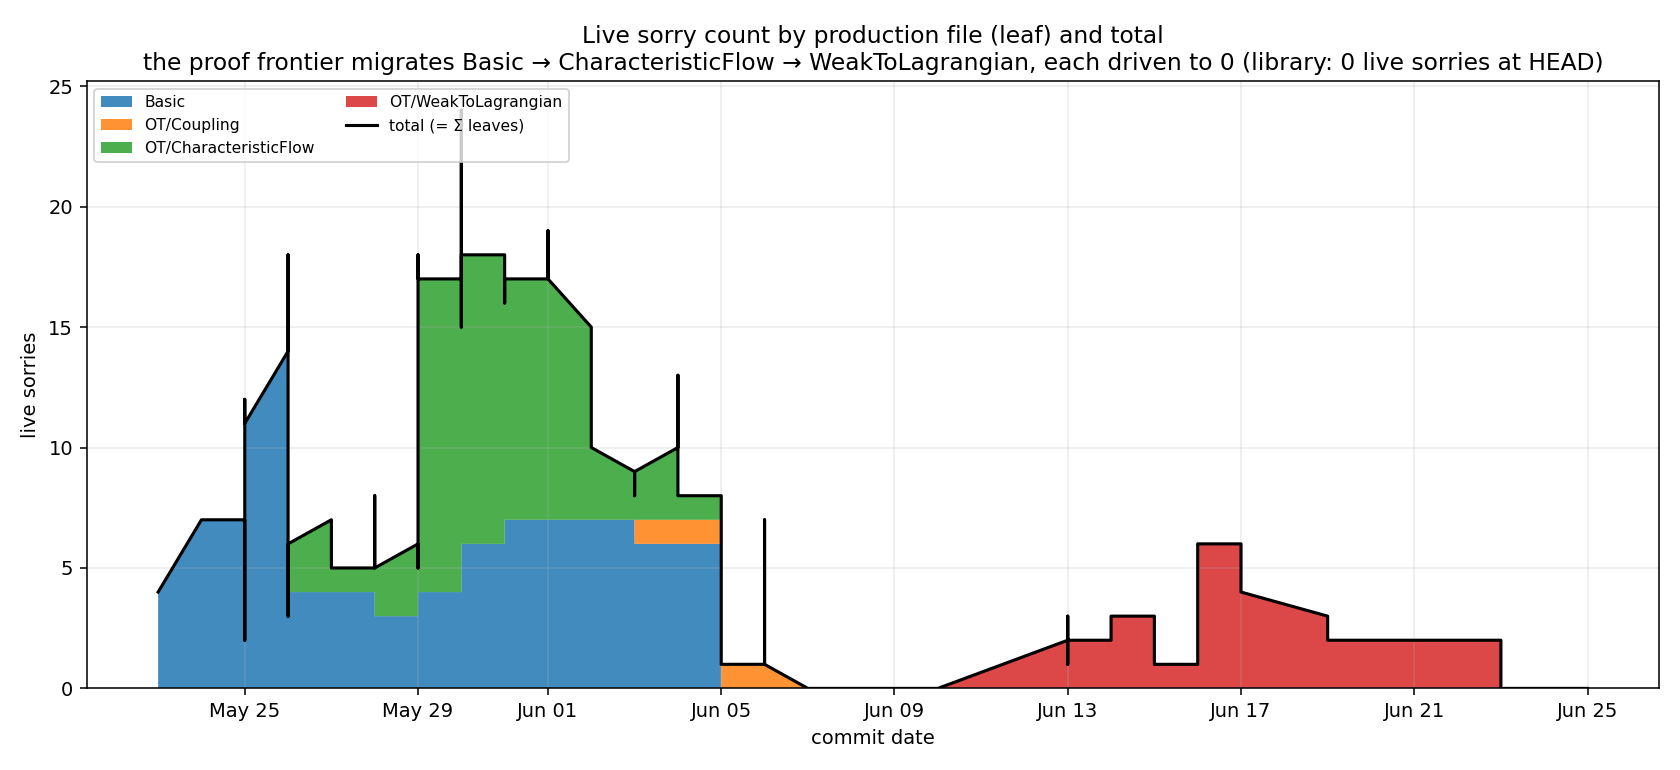
\includegraphics[width=\textwidth]{sorry_trajectory.png}
\caption{Live \lean{sorry} count per production file, stacked so the leaves sum to
the total (black line). The open-goal front is concentrated in one active leaf at a
time and migrates across the development; the total peaks at $24$ and returns to
$0$. The two humps are two games --- the well-posedness/stability marquee and the
superposition-principle follow-on --- separated by the zero-\lean{sorry} reusability
extraction.}
\label{fig:sorry}
\end{figure}

\subsection{The strategy taxonomy is earned, not designed}

Figure~\ref{fig:lessons} plots the standing instruction file's content over its
$36$ revisions: the count of named strategies present, split by series. The shape is
the visual signature of the central claim of Section~\ref{sec:strategies} --- that
the strategies were \emph{earned}, each keyed to a specific failure, rather than
designed in advance. The curve is a staircase: long flats punctuated by jumps where
a failure occurred and was distilled into a rule. The total grows from $4$ to $34$.
Two landmarks are legible: the four-series taxonomy itself crystallizes in a single
revision (before it, the file was an undifferentiated list of tool lessons; after,
all four series are present), and the process series jumps by four rules in one
revision --- the aftermath of exactly the cascade of frictions that the mid- and
end-game of Section~\ref{sec:phases} describe. The tool-lesson series keeps growing
through June, tracking the hardest analytic grind (the variational equation behind
the superposition bridge), and the framework stops growing once that crux closes:
$\mathcal{G}$ accumulates precisely when the game is hard, and is quiet when it is
not.

\begin{figure}[t]
\centering
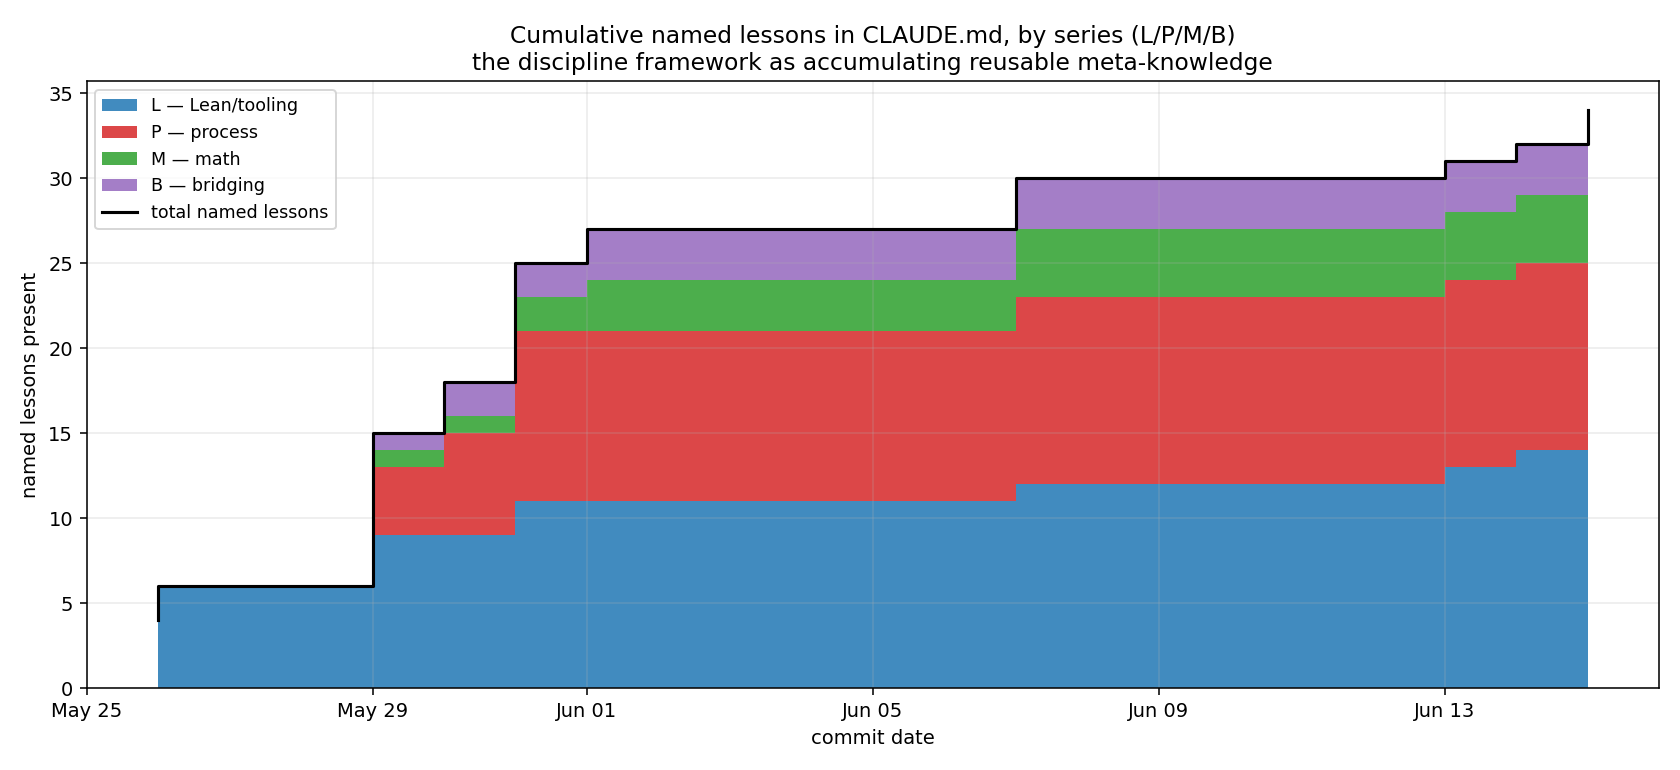
\includegraphics[width=\textwidth]{lessons_cumulative.png}
\caption{Named strategies present in the standing instruction file $\mathcal{G}$
across its $36$ revisions, by series (L/P/M/B; see Section~\ref{sec:strategies}).
The staircase shape --- flats punctuated by jumps at specific failures --- is the
signature of strategies earned rather than designed. The total grows $4\to34$; the
four-series taxonomy crystallizes in one revision, and the process (P) series jumps
by four in the aftermath of the cascade frictions of Section~\ref{sec:phases}.}
\label{fig:lessons}
\end{figure}

\subsection{The division of labor, counted}

Figure~\ref{fig:taxonomy} classifies all $362$ commits by primary intent. Just under
three-quarters are core proof work; the striking number is the second bar --- roughly
one commit in seven is pure meta-knowledge capture: editing the standing instruction
file, recording a strategy, or auditing the discipline. That fraction is a direct
measure of the meta-learning loop of Section~\ref{sec:strategies}: a substantial,
sustained share of the effort goes not into proving the next lemma but into
distilling \emph{how} the next lemma should be proved. The remainder is tooling and
documentation. The largest category being the proof itself, with meta-work a clear
and quantifiable second, is the division of labor of Section~\ref{sec:assessment}
seen from the commit log.

\begin{figure}[t]
\centering
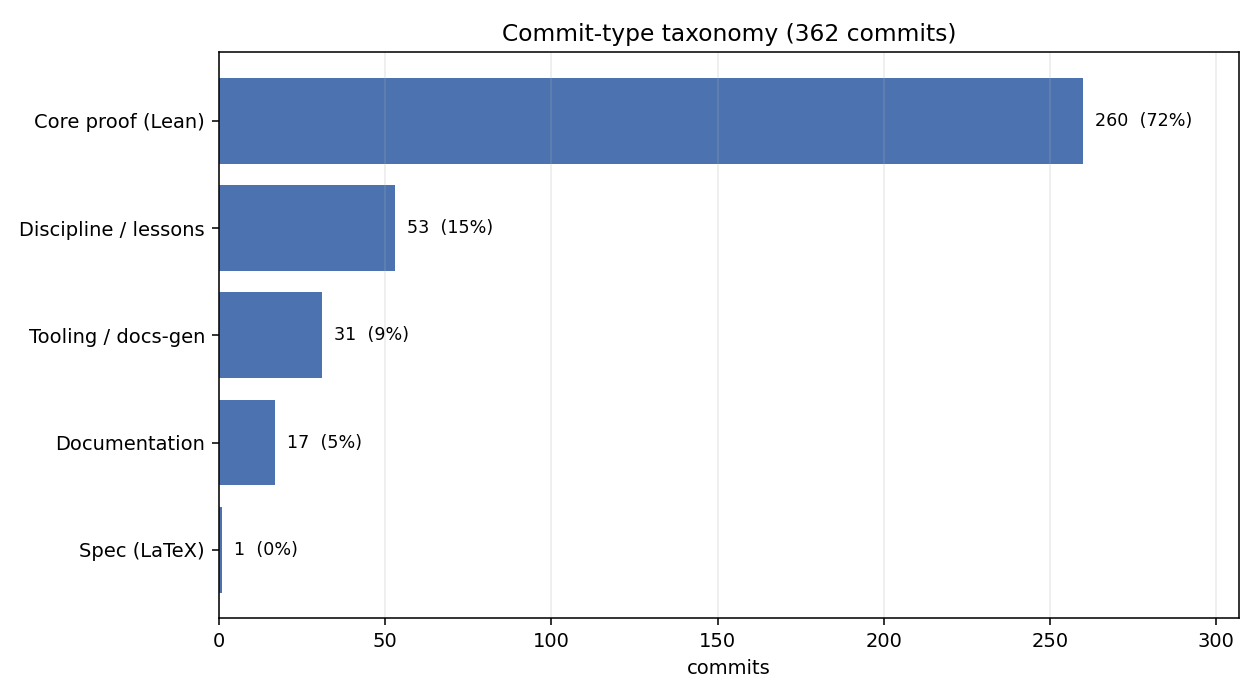
\includegraphics[width=0.86\textwidth]{commit_taxonomy.png}
\caption{All $362$ commits classified by primary intent. Roughly one in seven is
pure meta-knowledge capture (discipline / lessons) --- a direct, if heuristic,
measure of the meta-learning loop, distinct from the proof work itself.}
\label{fig:taxonomy}
\end{figure}

% ============================================================================
\section{Assessment}\label{sec:assessment}
% ============================================================================

\subsection{On ``about a week''}

The calendar span of the case study, from the first translated theorem to the
final certified extraction, was approximately one week. We state the figure
honestly, because the interesting claim is not raw speed but the \emph{mode} that
makes the speed possible.

This was neither solo human formalization (implausible at this speed for a result
of this size) nor autonomous AI formalization (which could not have made the
decomposition choices or the gap triage). It was a human mathematician acting as
strategic director over an AI execution engine: the human scoped the definitions,
chose the decompositions, triaged the library gaps, and accumulated the strategy
taxonomy; the agent executed the proofs, ran the builds, and handled the
mechanical sub-tasks. The week figure is evidence that this \emph{division of
labor} --- not either party alone --- has a real efficiency property, and the
verification discipline of Section~\ref{sec:discipline} is the reason the speed
did not come at the cost of soundness. The certification is the part that is not
a matter of trust: the target theorems' axiom footprints are \cleanfootprint,
and a referee can confirm this in seconds.

\subsection{What generalizes}

The case study is in kinetic theory, but the three-phase structure and the
strategy taxonomy are not specific to it. The early-game definitional-scoping
risk, the mid-game decomposition-is-human-judgment claim, and the endgame
library-gap triage should recur in any attempt to formalize research analysis,
where the rate-limiting resource is the ambient library's functional-analytic
coverage. The strategy series are stated at a level meant to transfer: the
P-series (process discipline) and B-series (bridging architecture) are
domain-independent; the M-series (mathematical structure) carries
analysis-flavored principles likely to recur in PDE formalization; the L-series
(tool idioms) is the most tool-specific and the most likely to age with the
proof assistant.

\subsection{Limitations and honest caveats}

The reusability score (Definition~\ref{def:score}) is defined and measured for
the case study, but we have not validated it across multiple developments; its
generality as a metric is a conjecture supported by one data point. The
``about a week'' figure is a single observation, not a controlled measurement,
and depends on the human director's prior fluency in both the mathematics and the
proof assistant. The strategy taxonomy was earned on one project and may be
incomplete; we expect later games to add series entries (the standing
instruction file is designed to keep accumulating them). Finally, one genuine
library gap in the case study (a Polish-space completeness fact for the
Wasserstein metric) was honestly \emph{deferred} as a cited placeholder rather
than built --- it lies off the path of the certified target theorems --- and is
recorded as such rather than papered over; a fully self-contained development
would build it, and it remains future work, most naturally as an upstream
contribution.

% ============================================================================
\section{Conclusion}
% ============================================================================

We have described AI-assisted Lean formalization as a strategy game with a
precise, machine-checkable win condition and a measurable reusability score, and
argued that the game has three phases --- definitional scoping, human-judgment
decomposition, and library-gap triage --- each rewarding a distinct strategy. The
human's role is not to write the proofs but to direct: to scope, to decompose, to
triage, and to accumulate strategic experience as standing guidance the agent
internalizes. We demonstrated the method by winning a substantial game --- a
complete, axiom-clean formalization of Vlasov well-posedness at arbitrary
interaction strength, with the mean-field stability and limit --- and by
extracting a reusable optimal-transport layer as the score. The certification is
the part that does not ask for trust: the target theorems depend on Lean's three
foundational axioms and nothing else, and the claim is checkable in seconds. We
believe the mathematician-in-the-loop framing, and the strategy taxonomy that
makes it operational, will transfer to other formalizations of research
analysis, where the human's mathematical judgment --- about how to cut a problem
and where the library runs out --- is exactly the scarce resource the loop is
designed to amortize.

\end{document}
